% ===================================================================
%  Week 7 — Morphological Image Processing — Session 1
% ===================================================================
\documentclass[10pt,aspectratio=169]{beamer}
% ===================================================================
%  Shared Beamer preamble for "Practical Image Processing"
%  English slides. Compile with pdfLaTeX.
% ===================================================================

\usetheme{metropolis}
\usepackage[T1]{fontenc}
\usepackage[utf8]{inputenc}
\usepackage{lmodern}
\usepackage{listings}
\usepackage{tcolorbox}
\usepackage{fontawesome5}
\usepackage{booktabs}
\usepackage{amsmath,amssymb}
\usepackage{tikz}
\usepackage{pgfplots}
\pgfplotsset{compat=1.17}
\usetikzlibrary{arrows.meta,positioning,shapes.geometric,fit,backgrounds,matrix}
\tcbuselibrary{skins,breakable}

% ---- Palette --------------------------------------------------------
\definecolor{coursePrimary}{HTML}{1B4965}   % deep blue
\definecolor{courseAccent}{HTML}{E76F51}    % coral
\definecolor{courseGood}{HTML}{2A9D8F}      % teal
\definecolor{courseBad}{HTML}{C0392B}       % red
\definecolor{courseInfo}{HTML}{2980B9}      % blue
\definecolor{codeBg}{HTML}{F5F6FA}
\definecolor{codeKw}{HTML}{8E44AD}
\definecolor{codeStr}{HTML}{2A9D8F}
\definecolor{codeCom}{HTML}{7F8C8D}

\setbeamercolor{frametitle}{bg=coursePrimary}
\setbeamercolor{progress bar}{fg=courseAccent}
\setbeamercolor{alerted text}{fg=courseAccent}
\metroset{block=fill,sectionpage=progressbar,numbering=fraction}

% ---- Code listings (Python is built into listings) -----------------
\lstdefinestyle{course}{
  backgroundcolor=\color{codeBg},
  basicstyle=\ttfamily\scriptsize,
  keywordstyle=\color{codeKw}\bfseries,
  stringstyle=\color{codeStr},
  commentstyle=\color{codeCom}\itshape,
  numberstyle=\tiny\color{codeCom},
  numbers=left, numbersep=6pt,
  showstringspaces=false, breaklines=true, breakatwhitespace=true,
  tabsize=4, columns=fullflexible,
  frame=single, framesep=4pt, rulecolor=\color{gray!30},
  keepspaces=true, upquote=true, language=Python,
}
\lstset{style=course}
\lstdefinelanguage{bash}{
  keywords={cd,pip,python,venv,source,import}, sensitive=true,
  morecomment=[l]{\#}, morestring=[b]', morestring=[b]",
}

% ---- Reusable callout boxes ----------------------------------------
\newtcolorbox{goodbox}[1][Good practice]{colback=courseGood!8,colframe=courseGood,
  fonttitle=\bfseries,title={\faCheck~#1},boxrule=0.6pt,left=4pt,right=4pt,top=3pt,bottom=3pt}
\newtcolorbox{badbox}[1][Pitfall]{colback=courseBad!8,colframe=courseBad,
  fonttitle=\bfseries,title={\faTimes~#1},boxrule=0.6pt,left=4pt,right=4pt,top=3pt,bottom=3pt}
\newtcolorbox{infobox}[1][Note]{colback=courseInfo!8,colframe=courseInfo,
  fonttitle=\bfseries,title={\faInfoCircle~#1},boxrule=0.6pt,left=4pt,right=4pt,top=3pt,bottom=3pt}
\newtcolorbox{mathbox}[1][Math]{colback=coursePrimary!6,colframe=coursePrimary,
  fonttitle=\bfseries,title={\faCalculator~#1},boxrule=0.6pt,left=4pt,right=4pt,top=3pt,bottom=3pt}

\newcommand{\keyidea}[1]{\begin{alertblock}{Key idea}#1\end{alertblock}}
\newcommand{\term}[1]{\textbf{\color{coursePrimary}#1}}
\newcommand{\code}[1]{\lstinline[basicstyle=\ttfamily\small]|#1|}

% ---- A helper to draw a small pixel grid, cells shaded by value ----
% \pixelgrid{ {10,20,120,200,240}, {30,60,130,180,230}, ... }
\newcommand{\pixelgrid}[1]{%
  \begin{tikzpicture}[font=\scriptsize,scale=0.6]
    \foreach \row [count=\ry] in {#1} {
      \foreach \val [count=\cx] in \row {
        \draw[gray,fill=coursePrimary!8] (\cx,-\ry) rectangle ++(1,-1);
        \node at (\cx+0.5,-\ry-0.5) {\val};
      }
    }
  \end{tikzpicture}}


\title{Morphological Processing}
\subtitle{Week 7 — Session 1: Erosion, dilation, opening \& closing}
\author{Practical Image Processing}
\date{Lecture 7.1 \textbullet\ 60--70 min}

\begin{document}

\maketitle

\begin{frame}{Recap \& today}
  \begin{columns}[T]
    \begin{column}{0.58\textwidth}
      \begin{itemize}
        \item Wk2/8: thresholding gives a \term{binary} image — but it is messy (specks, gaps, ragged edges).
        \item \alert{Today:} \term{morphology} — operations that grow, shrink, and clean binary shapes with a \term{structuring element}.
        \item Session 1 builds the four workhorses: \term{erosion}, \term{dilation}, \term{opening}, \term{closing}.
      \end{itemize}
    \end{column}
    \begin{column}{0.42\textwidth}
      \begin{alertblock}{DocScan milestone}
        After thresholding the meter digits, morphology removes noise and fills gaps so each digit is a clean, separable blob.
      \end{alertblock}
    \end{column}
  \end{columns}
\end{frame}

\begin{frame}{Roadmap}\tableofcontents\end{frame}

% ==================================================================
\section{The structuring element}
% ==================================================================

\begin{frame}{From smoothing to shape reasoning}
  \begin{itemize}
    \item Blurring \emph{averages} pixels; morphology \emph{compares} the shape of a small probe to the image.
    \item It works on a \term{binary} image (foreground = white = 1, background = black = 0).
    \item Every operation is built from two questions asked at each pixel: does the probe \emph{fit}, or does it \emph{hit}?
  \end{itemize}
  \begin{keyidea}{Morphology is shape surgery: it reasons about geometry, not brightness.}\end{keyidea}
\end{frame}

\begin{frame}{The structuring element (SE)}
  \begin{columns}[T]
    \begin{column}{0.55\textwidth}
      \begin{itemize}
        \item A small shape (the \term{SE} / kernel) that slides over the image — a probe with a chosen \term{anchor}.
        \item Common shapes: rectangle, ellipse, cross. Its \term{size} sets how aggressive the effect is.
        \item The anchor (usually the centre) is the pixel that receives the result.
      \end{itemize}
    \end{column}
    \begin{column}{0.45\textwidth}
      \begin{center}
      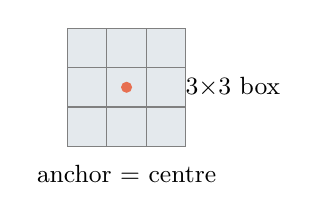
\begin{tikzpicture}[scale=0.5,font=\scriptsize]
        \foreach \x in {0,...,2}\foreach \y in {0,...,2}{
          \draw[gray,fill=coursePrimary!12] (\x,-\y) rectangle ++(1,-1);}
        \fill[courseAccent] (1.5,-1.5) circle (4pt);
        \node at (4.2,-1.5){\small $3{\times}3$ box};
        \node at (1.5,-3.7){\small anchor = centre};
      \end{tikzpicture}
      \end{center}
    \end{column}
  \end{columns}
\end{frame}

\begin{frame}[fragile]{Building an SE in OpenCV}
\begin{lstlisting}[language=Python]
import cv2
rect  = cv2.getStructuringElement(cv2.MORPH_RECT,    (3, 3))
ell   = cv2.getStructuringElement(cv2.MORPH_ELLIPSE, (5, 5))
cross = cv2.getStructuringElement(cv2.MORPH_CROSS,   (3, 3))
print(cross)   # 1s form a plus sign; 0s are ignored
\end{lstlisting}
  \begin{itemize}
    \item Only the \code{1} cells of the SE take part; the \code{0} cells are ignored.
    \item Odd sizes ($3,5,7,\dots$) keep a well-defined centre anchor.
  \end{itemize}
\end{frame}

% ==================================================================
\section{Erosion}
% ==================================================================

\begin{frame}{Erosion — the ``fit'' rule}
  \begin{itemize}
    \item Keep a foreground pixel \emph{only if} the SE fits \emph{entirely} inside the shape at that position.
    \item Effect: shapes \term{shrink}, thin protrusions vanish, and touching objects can \term{separate}.
    \item Formally $A \ominus B = \{z : B_z \subseteq A\}$ — the set of anchor positions where the shifted SE $B_z$ stays inside $A$.
  \end{itemize}
  \begin{mathbox}
    With a $3\times3$ box SE, a foreground pixel survives only if all 8 neighbours are also foreground.
  \end{mathbox}
\end{frame}

\begin{frame}{Erosion — worked $1$D-ish example}
  Foreground $=1$. Erode with a $1\times3$ horizontal SE (a pixel survives only if its left \emph{and} right neighbours are 1).
  \begin{columns}[T]
    \begin{column}{0.5\textwidth}\begin{center}
      {\scriptsize input row}\\[2pt]
      \pixelgrid{{0,1,1,1,0,1,0}}
    \end{center}\end{column}
    \begin{column}{0.5\textwidth}\begin{center}
      {\scriptsize after erosion}\\[2pt]
      \pixelgrid{{0,0,1,0,0,0,0}}
    \end{center}\end{column}
  \end{columns}
  \vspace{2pt}
  \begin{itemize}
    \item The lone $1$ dies (no neighbours); the run of three shrinks to its centre.
    \item Erosion removes objects thinner than the SE — that is how it deletes noise.
  \end{itemize}
\end{frame}

\begin{frame}{Erosion \& dilation on real digits}
  \begin{columns}[T]
    \begin{column}{0.33\textwidth}\begin{center}
      
\includegraphics[width=\linewidth]{../assets/binary.png}\\{\scriptsize binary digits}
    \end{center}\end{column}
    \begin{column}{0.33\textwidth}\begin{center}
      
\includegraphics[width=\linewidth]{../assets/erode.png}\\{\scriptsize erosion (thinner)}
    \end{center}\end{column}
    \begin{column}{0.33\textwidth}\begin{center}
      
\includegraphics[width=\linewidth]{../assets/dilate.png}\\{\scriptsize dilation (thicker)}
    \end{center}\end{column}
  \end{columns}
  \vspace{3pt}
  \begin{itemize}
    \item \term{Erosion}: strokes get thinner; hairline specks disappear entirely.
    \item \term{Dilation}: strokes get thicker; small gaps close up.
  \end{itemize}
\end{frame}

% ==================================================================
\section{Dilation}
% ==================================================================

\begin{frame}{Dilation — the ``hit'' rule}
  \begin{itemize}
    \item Set a pixel to foreground if the SE \emph{touches} (hits) the shape anywhere at that position.
    \item Effect: shapes \term{grow}, small holes and gaps fill, nearby pieces \term{connect}.
    \item Formally $A \oplus B = \{z : B_z \cap A \neq \varnothing\}$ — anchor positions where the shifted SE overlaps $A$.
  \end{itemize}
  \begin{mathbox}
    With a $3\times3$ box SE, a background pixel becomes foreground if \emph{any} of its 8 neighbours is foreground.
  \end{mathbox}
\end{frame}

\begin{frame}{Dilation — worked example}
  Dilate the same row with the $1\times3$ SE (a pixel becomes 1 if it \emph{or} a neighbour is 1).
  \begin{columns}[T]
    \begin{column}{0.5\textwidth}\begin{center}
      {\scriptsize input row}\\[2pt]
      \pixelgrid{{0,1,1,1,0,1,0}}
    \end{center}\end{column}
    \begin{column}{0.5\textwidth}\begin{center}
      {\scriptsize after dilation}\\[2pt]
      \pixelgrid{{1,1,1,1,1,1,1}}
    \end{center}\end{column}
  \end{columns}
  \vspace{2pt}
  \begin{itemize}
    \item Each run grows by one cell on each side; the one-cell gap between the runs is bridged.
    \item Dilation fills gaps smaller than the SE — that is how it repairs broken strokes.
  \end{itemize}
\end{frame}

\begin{frame}{Iterations vs a bigger SE}
  \begin{itemize}
    \item Two ways to make erosion/dilation stronger: a \emph{larger} SE, or \emph{more iterations} of a small SE.
    \item \code{iterations=n} applies the same SE $n$ times — cheap, and easy to tune interactively.
    \item Rough equivalence: $n$ passes of a $3\times3$ box $\approx$ one $(2n{+}1)\times(2n{+}1)$ box.
  \end{itemize}
  \begin{mathbox}
    Reach of erosion $\approx \lfloor k/2 \rfloor$ pixels for a $k\times k$ SE (per pass): a $5\times5$ box eats 2 pixels off every edge.
  \end{mathbox}
\end{frame}

\begin{frame}{Erosion and dilation are duals}
  \begin{itemize}
    \item Dilating the foreground $=$ eroding the background (and vice versa): $(A \ominus B)^c = A^c \oplus \hat{B}$.
    \item \term{Erosion} removes: thin protrusions, small objects; it \emph{separates} touching objects.
    \item \term{Dilation} adds: fills gaps, connects nearby pieces, \emph{thickens} thin strokes.
  \end{itemize}
  \begin{badbox}
    Each also distorts: erosion can break a thin digit; dilation can merge two close digits. Size matters — choose the smallest SE that works.
  \end{badbox}
\end{frame}

\begin{frame}{Neither preserves size — so we compose them}
  \begin{center}
  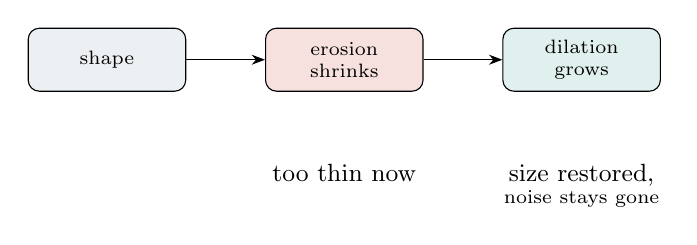
\begin{tikzpicture}[font=\scriptsize,>=Stealth,node distance=4mm and 10mm,
    b/.style={draw,rounded corners,fill=coursePrimary!8,minimum height=8mm,minimum width=20mm,align=center}]
    \node[b] (in){shape};
    \node[b,right=of in,fill=courseBad!15] (er){erosion\\shrinks};
    \node[b,right=of er,fill=courseGood!15] (di){dilation\\grows};
    \draw[->](in)--(er);\draw[->](er)--(di);
    \node[below=8mm of er,align=center]{\small too thin now};
    \node[below=8mm of di,align=center]{\small size restored,\\noise stays gone};
  \end{tikzpicture}
  \end{center}
  \begin{itemize}
    \item Raw erosion or dilation changes the object's size — often undesirable.
    \item Doing one then the \emph{other} (next section) cleans the shape while restoring its size.
  \end{itemize}
\end{frame}

% ==================================================================
\section{Opening \& closing}
% ==================================================================

\begin{frame}{Opening = erode then dilate}
  \begin{columns}[T]
    \begin{column}{0.5\textwidth}\begin{center}
      
\includegraphics[width=0.95\linewidth]{../assets/noisy.png}\\{\scriptsize binary + speckles}\\[4pt]
      
\includegraphics[width=0.95\linewidth]{../assets/open.png}\\{\scriptsize opening: specks gone}
    \end{center}\end{column}
    \begin{column}{0.5\textwidth}
      \begin{itemize}
        \item \term{Opening} removes small bright specks while keeping the digits' size: erosion kills the specks, dilation restores what remains.
        \item The classic ``clean up salt noise on a binary mask'' operation.
        \item $A \circ B = (A \ominus B) \oplus B$.
      \end{itemize}
    \end{column}
  \end{columns}
\end{frame}

\begin{frame}{Why opening keeps size but kills specks}
  \begin{itemize}
    \item A speck smaller than the SE is erased by the erosion and never comes back in the dilation.
    \item A digit larger than the SE is shrunk by erosion, then re-grown by dilation to (about) its original size.
    \item Geometric view: opening keeps exactly the parts where the SE could \emph{fully fit}, rolled along the shape.
  \end{itemize}
  \begin{goodbox}
    Opening is \term{idempotent}: applying it twice does nothing more than once. One well-sized pass is enough.
  \end{goodbox}
\end{frame}

\begin{frame}{Closing = dilate then erode}
  \begin{columns}[T]
    \begin{column}{0.5\textwidth}\begin{center}
      
\includegraphics[width=0.95\linewidth]{../assets/binary.png}\\{\scriptsize binary}\\[4pt]
      
\includegraphics[width=0.95\linewidth]{../assets/close.png}\\{\scriptsize closing: gaps filled}
    \end{center}\end{column}
    \begin{column}{0.5\textwidth}
      \begin{itemize}
        \item \term{Closing} fills small holes and gaps inside shapes while keeping the size.
        \item Repairs a digit broken by thresholding into a solid stroke.
        \item $A \bullet B = (A \oplus B) \ominus B$.
      \end{itemize}
    \end{column}
  \end{columns}
\end{frame}

\begin{frame}{Closing — worked example}
  Close the broken row with the $1\times3$ SE (dilate, then erode).
  \begin{center}
  \begin{tabular}{@{}rl@{}}
    input      & \pixelgrid{{1,1,0,1,1}}\\[6pt]
    dilate     & \pixelgrid{{1,1,1,1,1}}\\[6pt]
    then erode & \pixelgrid{{1,1,1,1,1}}\\
  \end{tabular}
  \end{center}
  \begin{itemize}
    \item The one-pixel gap is bridged by the dilation and \emph{survives} the erosion — the stroke is repaired.
    \item A gap wider than the SE would \emph{not} close: the SE size sets the maximum repairable gap.
  \end{itemize}
\end{frame}

\begin{frame}{The water-meter, step by step}
  \begin{center}
  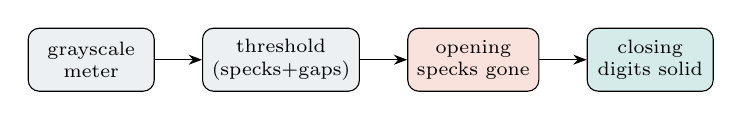
\begin{tikzpicture}[font=\scriptsize,>=Stealth,node distance=2mm and 6mm,
    b/.style={draw,rounded corners,fill=coursePrimary!8,minimum height=8mm,minimum width=16mm,align=center}]
    \node[b] (g){grayscale\\meter};
    \node[b,right=of g] (t){threshold\\(specks+gaps)};
    \node[b,right=of t,fill=courseAccent!20] (o){opening\\specks gone};
    \node[b,right=of o,fill=courseGood!20] (c){closing\\digits solid};
    \draw[->](g)--(t);\draw[->](t)--(o);\draw[->](o)--(c);
  \end{tikzpicture}
  \end{center}
  \begin{itemize}
    \item After thresholding, the ``7'' has a hairline break and a few salt specks float nearby.
    \item Opening deletes the specks; closing welds the ``7'' back into one stroke — now countable.
  \end{itemize}
  \begin{goodbox}
    This open-then-close pair is the core of the DocScan digit cleanup you will ship this week.
  \end{goodbox}
\end{frame}

\begin{frame}{Opening vs closing: remember the effect}
  \begin{center}
  \begin{tabular}{@{}lll@{}}
    \toprule
    \textbf{Operation} & \textbf{Order} & \textbf{Effect} \\
    \midrule
    Opening & erode $\rightarrow$ dilate & removes small \emph{bright} specks, breaks thin links \\
    Closing & dilate $\rightarrow$ erode & fills small \emph{dark} holes, bridges gaps \\
    \bottomrule
  \end{tabular}
  \end{center}
  \keyidea{Opening cleans the outside; closing repairs the inside. Both keep the overall size, unlike raw erosion/dilation.}
\end{frame}

% ==================================================================
\section{In-class exercise}
% ==================================================================

\begin{frame}{\faPen~In-class exercise (10 min)}
  \begin{infobox}[Pick the operation]
    For each defect on your thresholded meter, name the single morphology operation that fixes it — and the SE size you would start with.
  \end{infobox}
  \begin{enumerate}
    \item Scattered single white pixels (salt) around the digits.
    \item One digit is broken into two pieces by a threshold gap.
    \item Two adjacent digits are touching and need to be separated for counting.
    \item Trace the ``$0,1,1,0,1,1,1,0$'' row through erosion \emph{and} dilation with a $1\times3$ SE.
  \end{enumerate}
\end{frame}

\begin{frame}{\faPen~Debrief}
  \begin{itemize}
    \item (1) Salt specks $\rightarrow$ \term{opening} with a small ($3\times3$) SE.
    \item (2) Broken digit $\rightarrow$ \term{closing} sized just above the gap width.
    \item (3) Touching digits $\rightarrow$ careful \term{erosion} to separate (or watershed, Session 2 / Week 8).
    \item (4) Erode $\to 0,0,1,0,0,1,0,0$; \ dilate $\to 1,1,1,1,1,1,1,1$.
  \end{itemize}
  \keyidea{Diagnose the defect (specks / gaps / merges), then choose the matching operation and the smallest SE that fixes it.}
\end{frame}

% ==================================================================
\section{Wrap-up}
% ==================================================================

\begin{frame}{Common pitfalls}
  \begin{badbox}[Oversized SE]
    A too-large SE turns digits into unrecognizable blobs, or fuses neighbours. Tune the size on real data.
  \end{badbox}
  \begin{badbox}[Wrong polarity]
    On a \emph{white-on-black} mask, opening removes bright specks; if your foreground is inverted, open and close swap roles. Check which pixels are ``1''.
  \end{badbox}
\end{frame}

\begin{frame}[fragile]{The four operations in code}
\begin{lstlisting}[language=Python]
k = cv2.getStructuringElement(cv2.MORPH_ELLIPSE, (3, 3))
er = cv2.erode(binary, k, iterations=1)          # shrink
di = cv2.dilate(binary, k, iterations=1)         # grow
op = cv2.morphologyEx(binary, cv2.MORPH_OPEN,  k)  # remove specks
cl = cv2.morphologyEx(binary, cv2.MORPH_CLOSE, k)  # fill gaps
\end{lstlisting}
  \code{morphologyEx} wraps open/close (and more, next session) in one call.
\end{frame}

\begin{frame}{What you should now be able to do}
  \begin{itemize}
    \item Explain erosion/dilation via a structuring element (fit vs hit), and trace them by hand.
    \item Predict how the SE size changes the strength of each effect.
    \item Use opening (remove specks) and closing (fill gaps), and say why each preserves size.
  \end{itemize}
\end{frame}

\begin{frame}{Next session}
  \begin{infobox}[Session 2 preview]
    We build on erosion/dilation to get \term{gradient}, \term{top-hat}, and \term{black-hat}; extend morphology to \term{grayscale}; remove ruled lines while keeping text; and assemble the full DocScan cleanup pipeline.
  \end{infobox}
  \begin{itemize}
    \item Bring your thresholded meter image — we will clean it end-to-end.
  \end{itemize}
\end{frame}

\begin{frame}[standout]
  Threshold makes it binary; erosion and dilation reshape it.\\[4pt]
  \normalsize Opening removes specks, closing fills gaps — and both keep the size.
\end{frame}

\end{document}
